\section{Functions}
\textbf{Definition} A function is a correspondence between input numbers(x-values) and output numbers(y-values) such that each input number is paired with exactly one output number. \\
A non-mathematical example of a function is a vending machine. The input is the money(x-values) you put in and the output is the item you get(y-values). You can't put in the same amount of money and get two different items. \\

Functions can be described with an equation. 
\\
\textbf{Example}. $y = x^2 + 1$, which can also be written as $f(x) = x^2 + 1$. \\
\vspace{4pt}

What is $f(2)$ ? $ f(5) ?$ \\
\vspace{4pt}

When we write $f(2)$, we are asking what is the value of the function when $x = 2$. \\
So we take $2$ and plug it in for $x$ in the equation. \\

$$f(2) = 2^2 + 1 = 5$$
$$f(5) = 5^2 + 1 = 26$$ \\

Similarly, we can ask what is $f(a + 3)$
$$ f(a + 3) = (a+3)^2 + 1 = a^2 + 6a + 10 $$
\vspace{4pt}

We can also describe a function with a graph. \\
\textbf{Example}. The graph if $y = g(x)$ is shown below
\begin{align*}
    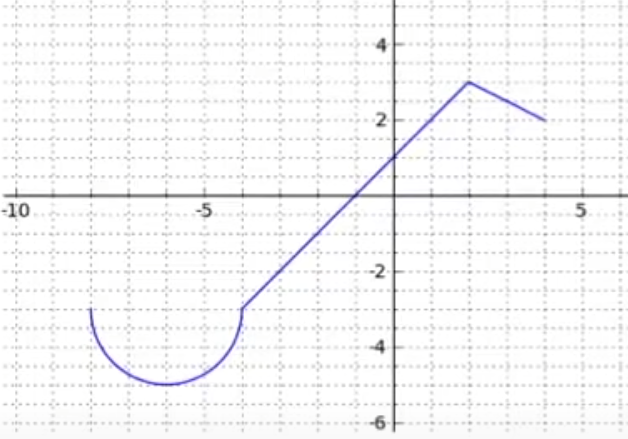
\includegraphics{algebra-pre-calculus/functions/graph1.png}
\end{align*}
\vspace{1pt}
What is $g(2)$ ? $ g(5) ?$ \\

First let's establish that $ y = g(x) $ so they are essentially mean the same thing. \\
In $g(2)$, $2$ corresponds to the $x$-value and we will use the graph to find corresponding $y$-value. \\
Since we know that we have to look for the $x$-value of $2$, we can look at the graph and find the point where $x = 2$. \\
Then we can look at the $y$-value of that point and that will be $3$. \\
Therefore, $g(2) = 3$. \\
Now when we look at $g(5)$, we can use the same method. However, we run into an issue that when we look at the x-value of $5$, we see that there is no point on the graph that has that x-value. \\
Therefore, $g(5)$ is undefined. \\
The question of what x-values and y-values makes sense to a function leads to the \textbf{domain} and \textbf{range} for a function. \\

\subsection{Domain and Range of a Function}
\textbf{Domain}: The domain of a function is the set of all possible x-values. \\
\textbf{Range}: The range of a function is the set of all possible y-values. \\

Let's examine the graph again and determine its range and domain. To find the domain of a function we have to look at the x-values that corresponds a point on the graph. \\
\begin{align*}
    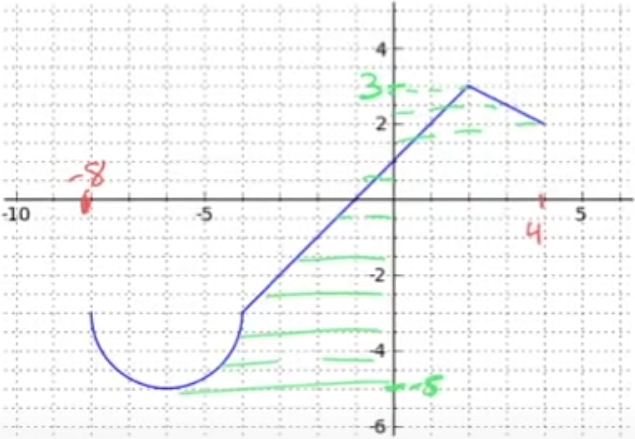
\includegraphics{algebra-pre-calculus/functions/graph2.png}
\end{align*}

We can see that the \textbf{domain} is $-8 \le x \le 4$. \\
Or as an interval notation, $[-8, 4]$. \\

To find the range of a function we have to look at the y-values that corresponds a point on the graph. \\
\textbf{range} is $-5 \le y \le 3$. \\
Or as an interval notation, $[-5, 3]$. \\

\subsection{Domain and Range of a Function as an Equation}
\textbf{Example}. Find the domain of these functions. \\
$\displaystyle A. \ g(x) = \frac{x}{x^2 - 4x + 3}$ \\
$\displaystyle B. \ f(x) = \sqrt{3-2x}$ \\
To find the domain of a function we have to consider algebraic restrictions. We can go ahead and question what values make sense to plug in for $x$. \\
Therefore, 
\begin{itemize}
    \item 1. Exclude x-values taht make the denominator 0. 
    \item 2. Exclude x-values that make the radicand(number under the radical) negative. Since we cannot take the square root of a negative number.
\end{itemize}